\documentclass{beamer}

\usepackage[utf8x]{inputenc}
\usepackage[OT4]{fontenc}

\setbeamertemplate{navigation symbols}{}

\usetheme[lang=pl,pasek=pasek2]{pwr}

\usepackage{ragged2e}
\usepackage{hyphenat}
\usepackage{hyperref}
\usepackage{booktabs}
\usepackage{listings}
\usepackage{multibib}

\usepackage{tikz}

\usetikzlibrary{arrows}
\usetikzlibrary{automata}
\usetikzlibrary{backgrounds}
\usetikzlibrary{decorations}

\usepackage{amsmath}
\usepackage{amsfonts}
\usepackage{amsthm}

\usepackage{highlight/pythonhighlight}

\title{
    Design and implementation issues \linebreak
    of a computer algebra system \linebreak
    in an interpreted, dynamically typed \linebreak
    programming language
}

\author{Mateusz Paprocki \texttt{<mattpap@gmail.com>}}
\institute[PWR]{Wrocław University of Technology}
\date{\today}

\newenvironment{jblock}[1]{
    \begin{block}{#1}\justifying\nohyphens
}{
    \end{block}
}

\setbeamercovered{transparent}

\begin{document}

\begin{frame}[plain,t]
    \maketitle
\end{frame}

\begin{frame}
    \frametitle{Wprowadzenie}
    \framesubtitle{}

    \begin{center}
        \structure{Design} and \structure{implementation} issues \linebreak
        of a \structure{computer algebra system} \linebreak
        in an \structure{interpreted}, dynamically typed \linebreak
        programming language
    \end{center}

    \begin{itemize}
        \item promotor: \structure{dr inż. Krzysztof Juszczyszyn}
        \item język realizacji pracy: \structure{angielski}
    \end{itemize}
\end{frame}

\begin{frame}
    \frametitle{Plan prezentacji}

    \begin{itemize}
        \item Wprowadzenie do SymPy
        \item Cele pracy dyplomowej
        \item Zrealizowane zadania
        \item Plany na przyszłość
    \end{itemize}
\end{frame}


\begin{frame}
    \frametitle{Co to jest SymPy?}
    \framesubtitle{}

    SymPy jest to \structure{biblioteka} pisana w \structure{Pythonie} do wykonywania:
    \begin{itemize}
        \pause
        \item obliczeń symbolicznych
            \begin{itemize}
                \item np. wyznaczanie całek, sum, granic
            \end{itemize}
        \pause
        \item \structure<5->{obliczeń algebraicznych}
            \begin{itemize}
                \item np. obliczanie baz Gr\"{o}bnera
            \end{itemize}
        \pause
        \item obliczeń numerycznych
            \begin{itemize}
                \item np. rozwiązywanie równań nieliniowych
            \end{itemize}
    \end{itemize}
\end{frame}

\begin{frame}
    \frametitle{Dlaczego SymPy?}
    \framesubtitle{}

    Dostępnych jest przecież wiele systemów matematycznych:
    \pause
    \begin{itemize}
        \item systemy \structure{zamknięte}:
            \begin{itemize}
                \item Mathematica, Maple, Magma, \ldots
            \end{itemize}
            \pause
        \item systemy \structure{otwarte}:
            \begin{itemize}
                \item Axiom, GiNaC, Maxima, PARI, Sage, Singular, Yacas, \ldots
            \end{itemize}
    \end{itemize}
    \pause
    Problemy:
    \begin{itemize}
        \item systemy \structure{wprowadzają} własny język programowania
            \begin{itemize}
                \item należy się taki język nauczyć od podstaw
                \item często jest to trudne zadanie, marnujemy czas
                \item \structure{wyjątki:} GiNaC i Sage
            \end{itemize}
            \pause
        \item występuje podział na:
            \begin{itemize}
                \item \structure{hermetyczne} i niedostępne jądro systemu
                \item biblioteki pisane w języku danego systemu
            \end{itemize}
    \end{itemize}
\end{frame}

\begin{frame}
    \frametitle{Co chcemy osiągnąć?}
    \framesubtitle{}

    \begin{itemize}
        \item biblioteka pisana w Pythonie
            \begin{itemize}
                \item bez nowego środowiska, języka, \ldots
                \item działa od razu na dowolnej platformie
                \item moduły nie--Pythonowe mogą być opcjonalne
            \end{itemize}
            \pause
        \item prostota architektury
            \begin{itemize}
                \item relatywnie mała baza kodu źródłowego
                \item łatwość w rozbudowie na dowolnym poziomie
            \end{itemize}
            \pause
        \item szeroka funkcjonalność
            \begin{itemize}
                \item obsługa najważniejszych działów matematyki
                \item wspieranie zaawansowanych metod i algorytmów
            \end{itemize}
            \pause
        \item użycie Cythona do optymalizacja wydajności
            \begin{itemize}
                \item opcjonalnie, jako dodatek do wersji interpretowanej
            \end{itemize}
            \pause
        \item liberalna licencja: BSD
            \begin{itemize}
                \item duża swoboda w użytkowaniu SymPy
            \end{itemize}
    \end{itemize}
\end{frame}

\begin{frame}
    \frametitle{Dlaczego wybraliśmy Pythona?}
    \framesubtitle{}

    \begin{itemize}
        \item prosty, interpretowany język programowania
            \begin{itemize}
                \item łatwa do nauczenia składnia i semantyka
                \item czytelny i łatwy w zarządzaniu kod
            \end{itemize}
            \pause
        \item język wykorzystywany przez potentatów
            \begin{itemize}
                \item Google, NASA, \ldots
            \end{itemize}
            \pause
        \item olbrzymia liczba bibliotek
            \begin{itemize}
                \item obliczenia numeryczne: NumPy, SciPy
                \item fizyka, symulacje, bioinformatyka
                \item wizualizacje 2D i 3D, wykresy
                \item bazy danych, narzędzia sieciowe, \ldots
            \end{itemize}
            \pause
        \item prostota łączenia ze światem zewnętrznym
            \begin{itemize}
                \item C/C++ poprzez natywne API lub Cythona
                \item Fortran poprzez bibliotekę f2py
            \end{itemize}
    \end{itemize}
\end{frame}

\begin{frame}
    \frametitle{Moja rola w projekcie}
    \framesubtitle{Czyli odrobina historii z moim udziałem}

    \begin{itemize}
        \item początek współpracy w marcu 2007 roku
            \begin{itemize}
                \item kilka prostych poprawek i rozszerzeń
            \end{itemize}
            \pause
        \item następnie Google Summer of Code 2007
            \begin{itemize}
                \item algorytmy rozwiązywania równań rekurencyjnych
                \item algorytmy sumowania nieznaczonego i oznaczonego
            \end{itemize}
            \pause
        \item no i tak już zostało:
            \begin{itemize}
                \item algorytmy całkowania symbolicznego
                \item struktury algebraiczne, wielomiany
                \item upraszczanie wyrażeń, \ldots
            \end{itemize}
            \pause
        \item poza tym:
            \begin{itemize}
                \item mentor w Google Summer of Code 2009 oraz 2010
                \pause
                \item prezentacja i krótki tutorial na EuroSciPy '09 (Lipsk)
                \pause
                \item prezentacja w ramach cyklu Py4Science (UC Berkely, 2010)
                \pause
                \item planowana prezentacja na EuroSciPy '10 (Paryż)
            \end{itemize}
    \end{itemize}
\end{frame}

\begin{frame}
    \frametitle{Cele pracy dyplomowej}
    \framesubtitle{}

    Zbudować moduł \structure{algebry komputerowej} dla SymPy:
    \begin{itemize}
        \item zgodnie z wymienionymi postulatami SymPy
        \pause
        \item szeroki wybór algorytmów i struktur danych
        \pause
        \item wprowadzenie architektury wielowarstwowej
        \pause
        \item wprowadzenie struktur algebraicznych
            \begin{itemize}
                \item wykorzystanie różnych typów bazowych
            \end{itemize}
        \pause
        \item wykorzystanie \structure{pure mode} Cython
        \pause
        \item \ldots
    \end{itemize}
\end{frame}

\begin{frame}
    \frametitle{Zaimplementowane algorytmy}
    \framesubtitle{}

    \begin{itemize}
        \item dekompozycja bezkwadratowa
            \begin{itemize}
                \item Yun
            \end{itemize}
        \item rozkład na czynniki proste
            \begin{itemize}
                \item nad ciałami skończonymi
                    \begin{itemize}
                        \item Berlekamp, Shoup, Zassenhaus
                    \end{itemize}
                \item nad innymi dziedzinami
                    \begin{itemize}
                        \item Cantor--Zassenhaus, Wang
                    \end{itemize}
            \end{itemize}
        \item dekompozycja funkcjonalna
            \begin{itemize}
                \item Landau--Zippel
            \end{itemize}
        \item bazy Gr\"{o}bnera
            \begin{itemize}
                \item Buchberger
            \end{itemize}
        \item izolacja pierwiastków
            \begin{itemize}
                \item ułamki łańcuchowe, Collins--Krandick
            \end{itemize}
    \end{itemize}
\end{frame}

\begin{frame}[fragile]
    \frametitle{Architektura wielowarstwowa}
    \framesubtitle{Poziomy L3 oraz L2}

    \begin{itemize}
        \item poziom L3
            \begin{python}
>>> f3 = x**10 - 1
>>> %timeit factor_list(f3)
100 loops, best of 3: 5.57 ms per loop
            \end{python}
            \pause
        \item poziom L2
            \begin{python}
>>> f2 = Poly(x**10 - 1, x, domain='ZZ')
>>> %timeit f2.factor_list()
100 loops, best of 3: 2.15 ms per loop
            \end{python}
    \end{itemize}
\end{frame}

\begin{frame}[fragile]
    \frametitle{Architektura wielowarstwowa}
    \framesubtitle{Poziomy L1 oraz L0}

    \begin{itemize}
        \item poziom L1
            \begin{python}
>>> f1 = DMP([1, 0, 0, 0, 0, 0, 0, 0, 0, 0, -1], ZZ)
>>> %timeit f1.factor_list()
100 loops, best of 3: 1.90 ms per loop
            \end{python}
            \pause
        \item poziom L0
            \begin{python}
>>> f0 = [1, 0, 0, 0, 0, 0, 0, 0, 0, 0, -1]
>>> %timeit dup_factor_list(f0, ZZ)
100 loops, best of 3: 1.88 ms per loop
            \end{python}
    \end{itemize}
\end{frame}

\begin{frame}
    \frametitle{Różne typy bazowe współczynników}
    \framesubtitle{Wprowadzenie}

    \begin{itemize}
        \item liczby całkowite $\mathbb{Z}$
            \begin{itemize}
                \item Python --- \texttt{int}
                \item SymPy --- \texttt{Integer}
                \item GMPY  --- \texttt{mpz}
                \item \ldots
            \end{itemize}
        \pause
        \item liczby wymierne $\mathbb{Q}$
            \begin{itemize}
                \item Python --- \texttt{Fraction}
                \item SymPy --- \texttt{Rational}
                \item GMPY  --- \texttt{mpq}
                \item \ldots
            \end{itemize}
        \pause
        \item inne dziedziny \ldots
    \end{itemize}
\end{frame}

\begin{frame}
    \frametitle{Różne typy bazowe współczynników}
    \framesubtitle{Benchmark}

    \begin{figure}
        \begin{center}
            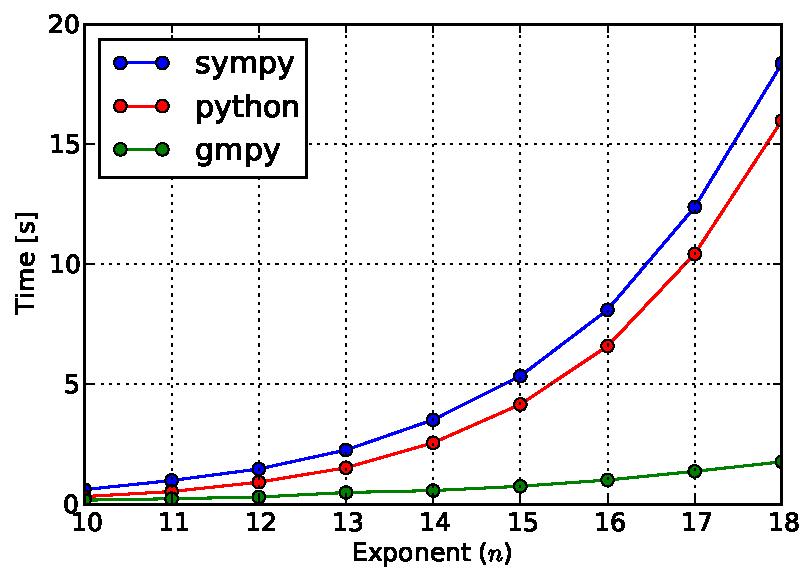
\includegraphics[scale=0.55]{images/ground-factor-large.pdf}
        \end{center}
        \caption{Rozkład na czynniki wielomianu $(1234 x + 123 y + 12 z + 1)^n$}
    \end{figure}
\end{frame}

\begin{frame}
    \frametitle{Plany na przyszłość}
    \framesubtitle{}

    \begin{itemize}
        \item zaangażowanie większej liczby osób w rozwój projektu
        \item więcej dokumentacji, przykładów, testów, benchmarków
        \item implementacja lepszych algorytmów
            \begin{itemize}
                \item algorytmy dekompozycji, bazy Gr\"{o}bnera, \ldots
            \end{itemize}
        \item zastosowanie modułu w praktyce
            \begin{itemize}
                \item projekt GSoC: Algorithms for Symbolic Integration
                \item wykorzystanie SymPy w zdalnej edukacji matematyki
            \end{itemize}
    \end{itemize}
\end{frame}

\begin{frame}
    \frametitle{Dziękuję za uwagę!}
    \framesubtitle{Pytania, uwagi, dyskusja \ldots}

    \begin{center}
        
\includegraphics[scale=0.2]{images/sympy-logo.pdf}
    \end{center}
\end{frame}

\end{document}

